% Created 2018-04-19 Thu 18:18
\documentclass[11pt]{article}
\usepackage[utf8]{inputenc}
\usepackage[T1]{fontenc}
\usepackage{fixltx2e}
\usepackage{graphicx}
\usepackage{longtable}
\usepackage{float}
\usepackage{wrapfig}
\usepackage{rotating}
\usepackage[normalem]{ulem}
\usepackage{amsmath}
\usepackage{textcomp}
\usepackage{marvosym}
\usepackage{wasysym}
\usepackage{amssymb}
\usepackage{hyperref}
\tolerance=1000
\usepackage{minted}
\author{Timothy Schwieg}
\date{\today}
\title{Econometrics Homework 9}
\hypersetup{
  pdfkeywords={},
  pdfsubject={},
  pdfcreator={Emacs 25.3.1 (Org mode 8.2.10)}}
\begin{document}

\maketitle
\section{Question 1}
\label{sec-1}
\subsection{a}
\label{sec-1-1}
\begin{align*}
L( \lambda | y ) = \prod_{n=1}^N \frac{  \lambda^{y_n} \exp{ - \lambda } }{ y_n ! }\\
f( \lambda ) = \sum_{n=1}^N y_n \log( \lambda ) - \lambda - \log( y_n ! )\\
g( \lambda ) = \sum_{n=1}^N \frac{ y_n }{ \lambda } - 1 = 0 \to \hat{\lambda} = \frac{1}{N} \sum_{n=1}^N y_n \\
\mathbb{V}[\hat{\lambda}] = \frac{1}{N^2} N \lambda = \frac{\lambda}{N}\\
\mathbb{E}[\hat{\lambda}] = \frac{1}{N} N \lambda = \lambda\\
\lim_{n \to \infty} \mathbb{V}[\hat{\lambda}] = 0. \text{ This implies
}\hat{\lambda}\text{ is consistent.}\\
\end{align*}

By the Lindinberg-Levy Central Limit theorem, the sample mean is
distributed approximately normally when adjusted appropiately. 

\begin{align*}
\hat{\lambda} \sim N( \lambda, \frac{\lambda}{N} )
\end{align*}

\begin{minted}[frame=lines,fontsize=\scriptsize,xleftmargin=\parindent,linenos,mathescape]{r}
library(ggplot2)
dataHorse <- read.table("PrussianArmy.dat", header=FALSE )

dataHorse <- dataHorse[order( dataHorse$V2 ),]

names(dataHorse) <- c("Year", "Corps", "V3" )

simpleGLM <- glm( formula= V3 ~ 1, family=poisson, data=dataHorse )

print( summary( simpleGLM ) )

print( exp(simpleGLM$coefficients[1] ) )

\end{minted}

\begin{verbatim}
Call:
glm(formula = V3 ~ 1, family = poisson, data = dataHorse)

Deviance Residuals: 
    Min       1Q   Median       3Q      Max  
-1.1832  -1.1832  -1.1832   0.3367   2.7099  

Coefficients:
            Estimate Std. Error z value Pr(>|z|)    
(Intercept) -0.35667    0.07143  -4.994 5.93e-07 ***
---
Signif. codes:  0 ‘***’ 0.001 ‘**’ 0.01 ‘*’ 0.05 ‘.’ 0.1 ‘ ’ 1

(Dispersion parameter for poisson family taken to be 1)

    Null deviance: 323.23  on 279  degrees of freedom
Residual deviance: 323.23  on 279  degrees of freedom
AIC: 630.31

Number of Fisher Scoring iterations: 5


(Intercept) 
        0.7 
\end{verbatim}



\subsection{b}
\label{sec-1-2}
\begin{minted}[frame=lines,fontsize=\scriptsize,xleftmargin=\parindent,linenos,mathescape]{r}
pdf("plot.pdf")

pot <-  ggplot( dataHorse, aes( x = 1:nrow(dataHorse), y = simpleGLM$residuals))
pot + geom_point( aes(color = Corps, shape = Corps )) + scale_shape_manual( values = 1:14 )

dev.off()
\end{minted}

\begin{figure}[htb]
\centering
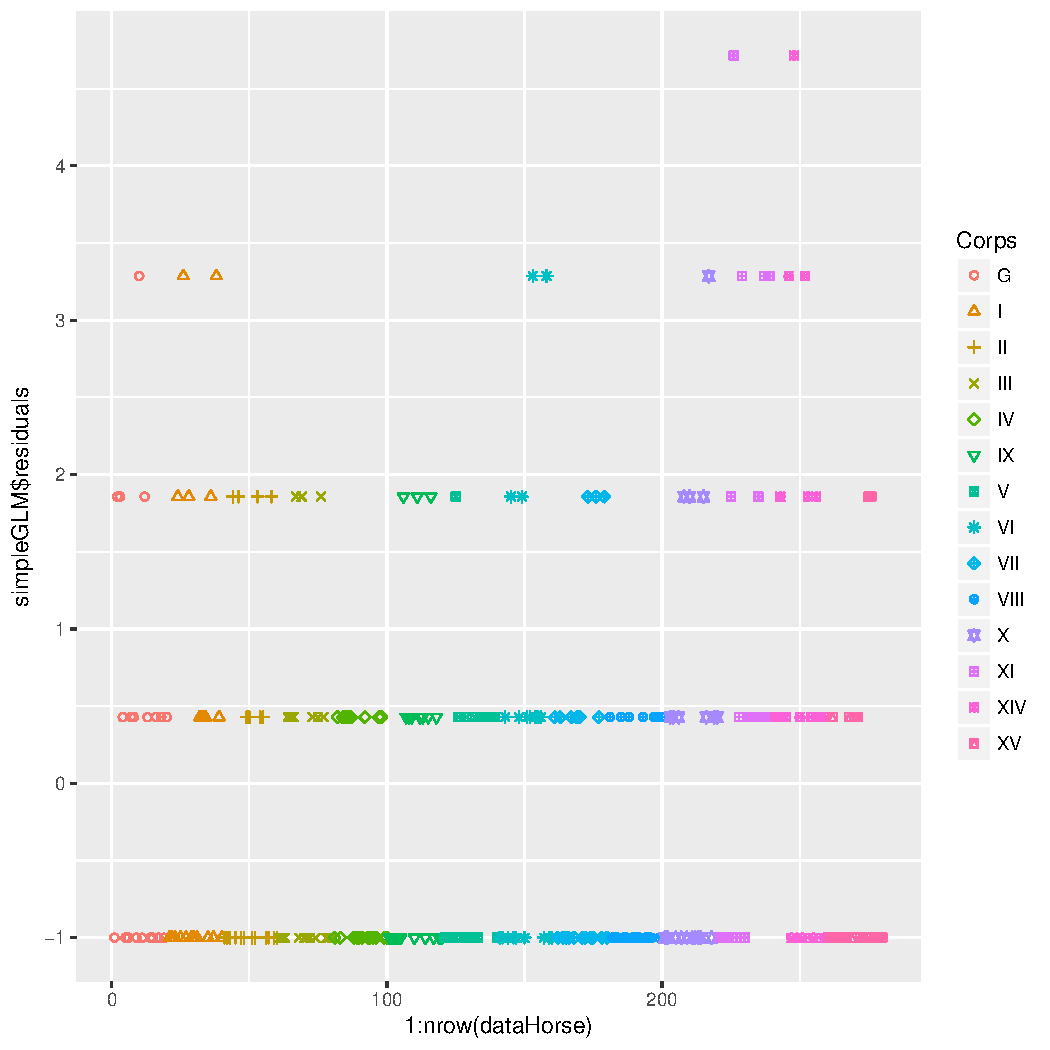
\includegraphics[width=.9\linewidth]{./plot.pdf}
\caption{Residuals controlled for Corps}
\end{figure}


\subsection{c}
\label{sec-1-3}
The vector \textbf{$\beta$} can be introduced using a link function and a single
index. The standard link function used in Poisson Regression is: $\log(\mu) =
X \beta$

The conditions for the maximum likelihood estimator is the standard
orthogonality condition for the Generalized Linear Model. This implies
that the residuals are orthogonal to the information. 
\begin{align*}
 X(  y - \exp{ X \beta  } ) = 0\\
\end{align*}

Since it is known that the mean of the distribution is $\lambda$, therefore we
may estimate this model by: $\lambda = \exp{ X \beta  }$

\begin{align*}
L( \lambda | y ) = \prod_{n=1}^N \frac{  \lambda^{y_n} \exp{ - \lambda } }{ y_n ! }\\
f( \lambda ) = \sum_{n=1}^N y_n X \beta   - \exp{ X \beta  } - \log( y_n ! )\\
\end{align*}

The maximum likelihood estimator is then given by taking the gradient
of this log-likelihood function and setting it equal to zero. The
system that follows is then solved by applying Newton's method until a
sufficient level of convergence has been reached.

\subsection{d}
\label{sec-1-4}
\begin{minted}[frame=lines,fontsize=\scriptsize,xleftmargin=\parindent,linenos,mathescape]{r}
lvl <- levels( dataHorse$Corps )
year <- unique( dataHorse$Year)

dummyData <- matrix(0, nrow = nrow(dataHorse), ncol = (length(lvl)+length(year)-1))

dummyData[,1] <- dataHorse[,3]

for( i in 2:length(lvl )){
    dummyData[,i] <- as.integer(dataHorse[,2] == lvl[i] )
}

for (i in 2:length(year)){
    dummyData[,length(lvl)+i-1] <- as.integer( dataHorse[,1] == year[i] )
}

complexGLM <- glm( formula=X1~., family=poisson, data=data.frame(dummyData) )

print( summary( complexGLM ) )


pValue <- pchisq( 2*(logLik(complexGLM) - logLik(simpleGLM )), df = 32,lower.tail = FALSE )
print( pValue )
\end{minted}

\begin{verbatim}
Call:
glm(formula = X1 ~ ., family = poisson, data = data.frame(dummyData))

Deviance Residuals: 
    Min       1Q   Median       3Q      Max  
-1.7671  -0.9897  -0.6185   0.5655   1.9776  

Coefficients:
              Estimate Std. Error z value Pr(>|z|)   
(Intercept) -1.407e+00  6.251e-01  -2.251  0.02440 * 
X2           3.295e-16  3.536e-01   0.000  1.00000   
X3          -2.877e-01  3.819e-01  -0.753  0.45125   
X4          -2.877e-01  3.819e-01  -0.753  0.45125   
X5          -6.931e-01  4.330e-01  -1.601  0.10943   
X6          -2.076e-01  3.734e-01  -0.556  0.57815   
X7          -3.747e-01  3.917e-01  -0.957  0.33875   
X8           6.062e-02  3.483e-01   0.174  0.86183   
X9          -2.877e-01  3.819e-01  -0.753  0.45125   
X10         -8.267e-01  4.532e-01  -1.824  0.06812 . 
X11         -6.454e-02  3.594e-01  -0.180  0.85749   
X12          4.463e-01  3.202e-01   1.394  0.16333   
X13          4.055e-01  3.227e-01   1.256  0.20901   
X14         -6.931e-01  4.330e-01  -1.601  0.10943   
X15          5.108e-01  7.303e-01   0.699  0.48425   
X16          8.473e-01  6.901e-01   1.228  0.21950   
X17          1.099e+00  6.667e-01   1.648  0.09937 . 
X18          1.204e+00  6.583e-01   1.829  0.06740 . 
X19          1.792e+00  6.236e-01   2.873  0.00406 **
X20          6.931e-01  7.071e-01   0.980  0.32696   
X21          1.540e+00  6.362e-01   2.421  0.01547 * 
X22          1.299e+00  6.513e-01   1.995  0.04607 * 
X23          1.099e+00  6.667e-01   1.648  0.09937 . 
X24          5.108e-01  7.303e-01   0.699  0.48425   
X25          1.299e+00  6.513e-01   1.995  0.04607 * 
X26          1.609e+00  6.325e-01   2.545  0.01094 * 
X27          6.931e-01  7.071e-01   0.980  0.32696   
X28          1.299e+00  6.513e-01   1.995  0.04607 * 
X29          1.735e+00  6.262e-01   2.770  0.00561 **
X30          1.386e+00  6.455e-01   2.148  0.03174 * 
X31          1.609e+00  6.325e-01   2.545  0.01094 * 
X32          9.808e-01  6.770e-01   1.449  0.14740   
X33          2.877e-01  7.638e-01   0.377  0.70642   
---
Signif. codes:  0 ‘***’ 0.001 ‘**’ 0.01 ‘*’ 0.05 ‘.’ 0.1 ‘ ’ 1

(Dispersion parameter for poisson family taken to be 1)

    Null deviance: 323.23  on 279  degrees of freedom
Residual deviance: 258.59  on 247  degrees of freedom
AIC: 629.67

Number of Fisher Scoring iterations: 6


'log Lik.' 0.0005523346 (df=33)
\end{verbatim}

Based on the p-value taken from a likelhood ratio test, we find it
very unlikely that none of the variables matter, as the probability of
all these deviations being caused by noise is extremely small. 
% Emacs 25.3.1 (Org mode 8.2.10)
\end{document}